%% Copyright 2007 Ulf Lindgren
%
% This work may be distributed and/or modified under the conditions of the LaTeX
% Project Public License, either version 1.3 of this license or (at your option)
% any later version. The latest version of this license is in
%   http://www.latex-project.org/lppl.txt
% and version 1.3 or later is part of all distributions of LaTeX version
% 2005/12/01 or later.
%
% This work has the LPPL maintenance status `maintained'.
% 
% The Current Maintainer of this work is Ulf Lindgren.
%
% This work consists of all files listed in manifest.txt.
%
%% This statement added 2010/12/10 by Clea F. Rees following correspondence
%% between Ulf Lindgren and Karl Berry concerning licensing.

\documentclass{report}

  \usepackage[body={16cm,23cm}]{geometry} % Pour remplacer les réglages manuels
  \usepackage[T1]{fontenc}
  \usepackage[inputenc,babel]{translatex-fr}
  \usepackage{graphicx}
  \usepackage[Lenny]{fncychap}
  \usepackage{lettrine} % Pour remplacer ydrop qui ne donne pas les résultats attendus.

  \newcommand{\sk}{\vspace{0.2 cm}}
  \newcommand{\A}[1]{{$\backslash${\tt #1}}}
  \newcommand{\nsp}{\mbox{\hspace{-1 cm}}}
  \title{L'extension FncyChap\\V1.34}
  \author{Ulf A. Lindgren}
  \date{}

\begin{document}
  \maketitle
  \tableofcontents
  \chapter{Description de l'extension}
    \lettrine[findent=0.2em,nindent=0em,realheight=true]{L'}{extension} 
    \textsl{fncychap} a été écrite afin que des titres de niveau chapitre
    puissent être altérés rapidement et que je puisse apprendre plus sur
    \TeX{} et \LaTeX{}. Je ne sais pas si cette extension est écrite de façon
    adéquate. Aussi, si quelqu'un lit cette documentation et essaye 
    \textsl{fncychap}, je serais reconnaissant pour tout retour d'expérience. 
    Ceci m'aidera à monter compétence dans l'écriture de commandes. 
 
    Dans toute publication, il est essentiel de se rappeler que la cohérence
    joue un rôle important. Ainsi, avec cette extension, il est possible de
    modifier l'apparence de chaque chapitre séparément dans un document. Ceci
    n'est cependant pas souhaitable : n'oubliez ici pas la modestie et la 
    cohérence.

    \section{Chargement et utilisation classique}
    Cette extension est chargée en saisissant la ligne suivante en 
    préambule\sk\\    
    \nsp\fbox{\A{usepackage}[{\em style}]\{{\em fncychap}\}}\sk\\    
    Si l'option \emph{style} est omise alors la définition par défaut des 
    chapitres est utilisée. À l'origine, il existait six styles de chapitres
    prédéfinis, à savoir \emph{Sonny, Lenny, Glenn, Conny, Rejne} et 
    \emph{Bjarne}. Ces noms correspondent à des prénoms suédois, à l'image sans
    doute d'IKEA\footnote{Marque déposée d'Ingvar Kamprad Emtaryd Agunnaryd.}. 
    Chacun de ces styles dispose d'une configuration par défaut et, si elle
    est suffisante, il ne reste rien d'autre à faire.

    Dans la version actuelle de \textsl{fncychap}, deux styles additionnels
    ont été ajoutés. Le premier se nomme \emph{PetersLenny}, d'après le nom de
    son auteur Peter Osborn. Ce style se base sur celui de \emph{Lenny} : Peter
    a finement ajusté la taille des filets pour chacun des chapitres numérotés
    (jusqu'à 20) et chacune des annexes (jusqu'à Z). Le second style a été 
    défini par Jean-Marc François et il l'a nommé \textsl{Bjornstrup}.

    À l'origine, \textsl{fncychap} ne dépendait d'aucune autre extension. 
    Cependant, pour le style {\tt Lenny}, une fonte postscript est utilisée
    par défaut ; mais ceci peut être facilement changé. J'encourage 
    l'utilisation de cette fonte postscript par défaut car elle est 
    redimensionnable de façon très importante, ce qui rend \emph{Lenny} 
    très agréable. Dans la version actuelle, si le style \textsl{Bjornstrup}
    de Jean-Marc est utilisé, l'extension \textsl{color} de la distribution de
    base sera chargée. 
    
  \chapter{Nouvelles commandes}
    \lettrine[findent=0.2em,nindent=0em,realheight=true]{E}{n} parallèle des 
    styles de chapitre, quelques commandes additionnelles sont mises à 
    disposition afin de créer ses titres de chapitre personnalisés.
    Les commandes vont être décrites les unes à la suite des autres. Chaque
    commande est encadrée et placée sur une ligne séparée. Commençons donc 
    ces descriptions.\sk\\
    \nsp\fbox{\A{mghrulefill}\{{\em largeur}\}}\sk\\
    La commande ci-dessus est une version plus générale de la commande
    \A{hrulefill} dans le sens où la largeur du filet peut être spécifiée.
    Cette commande est fournie pour décorer les titres de chapitre. Les
    titres se divisent en deux parties. La première définit \A{chapapp} 
    contenant le texte \og Chapter \fg{}\footnote{N.D.T. : avec le chargement
    de \textsl{color} et de son option \texttt{french}, ce texte est 
    \og Chapitre \fg{}.} ainsi que \A{thechapter} contenant le numéro du
    chapitre. La seconde partie est le titre du chapitre donné par 
    l'utilisateur. À partir d'ici, \A{chapapp} et \A{thechapter} seront
    respectivement nommé nom du chapitre et numéro du chapitre. Le titre
    donné par l'utilisateur sera nommé titre du chapitre.

    \section{Vers la personnalisation du titre de chapitre}
    \label{sec:TW}
    Les nom, numéro et titre du chapitre peuvent être changés simplement. 
    Introduisons ici les deux commandes suivantes :\sk\\
    \nsp\fbox{\A{ChNameUpperCase} et \A{ChNameLowerCase}}\sk\\
    qui passent respectivement le nom du chapitre en lettres majuscules
    (\emph{uppercase}) ou en lettres minuscules (\emph{lowercase}). Un
    cas particulier est ajouté pour le nom du chapitre, à savoir\sk\\
    \nsp\fbox{\A{ChNameAsIs}}\sk\\
    qui affiche le format par défaut. Trois commandes similaires existent pour
    le titre du chapitre \sk\\
    \nsp\fbox{\A{ChTitleUpperCase}, \A{ChTitleLowerCase} et
      \A{ChNameAsIs}}\sk\\
    La largeur du filet des styles de chapitre prédéfinis peut être contrôlée
    par la commande\sk\\
    \nsp\fbox{\A{ChRuleWidth}\{{\em largeur}\}}\sk\\
    en gardant en tête que la {\em largeur} doit avoir une unité, par exemple
    {\em pt, mm}, etc. Les éléments liés aux polices de caractères tels que la
    police, son corps, sa graisse peuvent être transmis par les commandes\sk\\
    \nsp\fbox{\A{ChNameVar}\{{\em argument}\}, \A{ChNumVar}\{{\em argument}\} 
    et \A{ChTitleVar}\{{\em argument}\}}\sk\\
    liées respectivement aux nom, numéro et titre du chapitre. L{\em 'argument}
    de ces fonctions peut être par exemple 
    \mbox{\A{ChNameVar}\{\A{huge}\A{rm}\A{centering}\}}.


  \chapter{Aperçu des styles de chapitre}
    \lettrine[findent=0.2em,nindent=0em,realheight=true]{L}{es} styles de 
    chapitre ont tous des réglages par défaut pour chacune des commandes
    décrites en section~\ref{sec:TW}. Cependant, ils peuvent être changés
    en recourant à ces commandes. Notez que si \A{centering}, etc. est 
    utilisé pour mettre en forme le titre de chapitre, cela peut conduire
    à des résultats affreux. Le style de chapitre \emph{Bjarne} contient 
    une commande complémentaire\sk\\
    \nsp\fbox{\A{TheAlphaChapter}}\sk\\
    Cette commande écrit le numéro du chapitre en utilisant les mots 
    équivalents. \A{TheAlphaChapter} peut écrire les nombres de
    emph{ZERO} to \emph{NINETYNINE}\footnote{N.D.T. : dans un texte français,
    il faut redéfinir la commande \A{TheAlphaChapter} ainsi que la 
    commande \A{AlphaNo} pour remplacer les termes anglais par des termes 
    français.}.
    
    Dans les sections suivantes, les styles prédéfinis sont présentés en 
    compagnie de leur paramétrage par défaut. Les versions \A{chapter} 
    et \A{chapter*} (dite \og étoilée \fg{}) sont toutes deux illustrées.

    \section{Le style de chapitre Sonny}
    Les paramètres par défaut sont les suivants :
    {\small\begin{verbatim}  
     \ChNameVar{\Large\sf}  \ChNumVar{\Huge}  \ChTitleVar{\Large\sf}
     \ChRuleWidth{0.5pt}    \ChNameUpperCase
    \end{verbatim}}    
    \begin{figure}[h]
      \begin{minipage}{7 cm}
        \label{fig:Sonnys}
        \centerline{\includegraphics[height=6cm]{Sonnys.eps}} 
        \caption{Le style Sonny \og étoilé \fg{}}
      \end{minipage}\hfill
      \begin{minipage}{7 cm}
        \label{fig:Sonny}
        \centerline{\includegraphics[height=6cm]{Sonny.eps}}
        \caption{Le style Sonny}
      \end{minipage}\hfill
    \end{figure}    
    
    \section{Le style de chapitre Lenny}
    Les paramètres par défaut sont les suivants :
    {\small\begin{verbatim}
     \ChNameVar{\fontsize{14}{16}\usefont{OT1}{phv}{m}{n}\selectfont}
     \ChNumVar{\fontsize{60}{62}\usefont{OT1}{ptm}{m}{n}\selectfont}
     \ChTitleVar{\Huge\bfseries\rm}  \ChRuleWidth{1pt}
    \end{verbatim}}
    \begin{figure}[h]
      \begin{minipage}{7 cm}
        \centerline{\includegraphics[height=6cm]{Lennys.eps}} 
        \caption{Le style Lenny \og étoilé \fg{}}
      \end{minipage}\hfill
      \begin{minipage}{7 cm}
        \centerline{\includegraphics[height=6cm]{Lenny.eps}}
        \caption{Le style Lenny}
      \end{minipage}\hfill
    \end{figure}
    \textbf{Note:} Une version alternative nommée \textsl{PetersLenny} existe.

    \section{Le style de chapitre Glenn}
    Les paramètres par défaut sont les suivants :
    {\small\begin{verbatim}
     \ChNameVar{\bfseries\Large\sf}  \ChNumVar{\Huge}  \ChTitleVar{\bfseries\Large\rm}, 
     \ChRuleWidth{1pt}               \ChNameUpperCase  \ChTitleUpperCase
    \end{verbatim}}
    \begin{figure}[h]
      \begin{minipage}{7 cm}
        \centerline{\includegraphics[height=6cm]{Glenns.eps}}
        \caption{Le style Glenn \og étoilé \fg{}}
      \end{minipage}\hfill
      \begin{minipage}{7 cm}
        \centerline{\includegraphics[height=6cm]{Glenn.eps}}
        \caption{Le style Glenn}
      \end{minipage}\hfill
    \end{figure}

    \section{Le style de chapitre Conny}
    Les paramètres par défaut sont les suivants :
    {\small\begin{verbatim}
     \ChNameUpperCase     \ChTitleUpperCase    \ChNameVar{\centering\Huge\rm\bfseries}
     \ChNumVar{\Huge}     \ChRuleWidth{2pt}    \ChTitleVar{\centering\Huge\rm}
    \end{verbatim}}
    \begin{figure}[h]
      \begin{minipage}{7 cm}
        \centerline{\includegraphics[height=6cm]{Connys.eps}}
        \caption{Le style Conny \og étoilé \fg{}}
      \end{minipage}\hfill
      \begin{minipage}{7 cm}
        \centerline{\includegraphics[height=6cm]{Conny.eps}}
        \caption{Le style Conny}
      \end{minipage}\hfill
    \end{figure}

    \section{Le style de chapitre Rejne}
    Les paramètres par défaut sont les suivants :
    {\small\begin{verbatim}  
     \ChNameVar{\centering\Huge\rm\bfseries} \ChNumVar{\Huge}  \ChTitleVar{\centering\Huge\rm}
     \ChNameUpperCase                        \ChTitleUpperCase \ChRuleWidth{1pt}
    \end{verbatim}}
    \begin{figure}[h]
      \begin{minipage}{7 cm}
        \centerline{\includegraphics[height=6cm]{Rejnes.eps}}
        \caption{Le style Rejne \og étoilé \fg{}}
      \end{minipage}\hfill
      \begin{minipage}{7 cm}
        \centerline{\includegraphics[height=6cm]{Rejne.eps}}
        \caption{Le style Rejne}
      \end{minipage}\hfill
    \end{figure}

    \section{Le style de chapitre Bjarne}
    Les paramètres par défaut sont les suivants :
    {\small\begin{verbatim}
     \ChNameUpperCase   \ChNameVar{\raggedleft\normalsize\rm}   \ChRuleWidth{1pt}
     \ChTitleUpperCase  \ChNumVar{\raggedleft \bfseries\Large} 
     \ChTitleVar{\raggedleft \Large\rm}
    \end{verbatim}}
    \begin{figure}[h]
      \begin{minipage}{7 cm}
        \centerline{\includegraphics[height=6cm]{Bjarnes.eps}} 
        \caption{Le style Bjarne \og étoilé \fg{}}
      \end{minipage}\hfill
      \begin{minipage}{7 cm}
        \centerline{\includegraphics[height=6cm]{Bjarne.eps}}
        \caption{Le style Bjarne}
      \end{minipage}\hfill
    \end{figure}

    \section{Le style de chapitre Bjornstrup}
    Les paramètres par défaut sont les suivants :
    {\small\begin{verbatim}
     \ChNumVar{\fontsize{76}{80}\usefont{OT1}{pzc}{m}{n}\selectfont}
     \ChTitleVar{\raggedleft\Large\sffamily\bfseries}
    \end{verbatim}}
    \begin{figure}[h]
      \begin{minipage}{7 cm}
        \centerline{\includegraphics[height=6cm]{BjornstrupS.eps}} 
        \caption{Le style Bjornstrup \og étoilé \fg{}}
      \end{minipage}\hfill
      \begin{minipage}{7 cm}
        \centerline{\includegraphics[height=6cm]{Bjornstrup.eps}}
        \caption{Le style Bjornstrup}
      \end{minipage}\hfill
    \end{figure}
    \textbf{Note:} la restitution faite par YAP (visualisateur dvi de MikTeX)
    diffère de dvips dans la mesure où la boîte grise passe au premier plan et
    cache ainsi une partie du numéro de chapitre. 
    \enlargethispage{2cm}


  \chapter{Exemple simple}
    \lettrine[findent=0.2em,nindent=0em,realheight=true]{S}{i} les styles
    prédéfinis ne répondent pas à vos besoins, vous pouvez modifier les
    routines de mise en forme. Cette mise en forme est contrôlée par trois
    commandes.
    \tradini
    One might as well redefine the original
    chapter definitions using the \A{secdef} and \A{renewcommand}, see
    The \LaTeX{} companion. However, at the time of creating this
    package I decided that this was easier. The command\sk\\
    \nsp\fbox{\A{DOCH}}\sk\\
    formats the chapter name and number. The commands\sk\\
    \nsp\fbox{\A{DOTI}\{{\#1}\}}\sk\\
    and\sk\\
    \nsp\fbox{\A{DOTIS}\{{\#1}\}}\sk\\
    formats the chapter title for \A{chapter} and \A{chapter*} respectively.
    In order to modify these you will have to use the preamble along
    with the commands \A{makeatletter} and \A{makeatother}. The in
    addition some predefined parameters can be used. The predefined
    length variables are\sk\\
    \nsp\fbox{\A{mylen}, \A{myhi}, \A{px}, \A{py}, \A{pxx}, \A{pyy}
      and \A{RW}}\sk\\
    note that \A{RW} is special, since it is set by \A{ChRuleWidth}.
    The formatting controlled by \A{ChNameVar}, \A{ChNumVar} and
    \A{ChTitleVar} store their values in \A{CNV}, \A{CNoV} and \A{CTV}
    respectively. Finally, The functions \A{FmN}\{ \} and \A{FmTi}\{
    \} acts accordingly to \A{Ch***AsIs}, \A{Ch***UpperCase} and
    \A{Ch***LowerCase}. Note that the stars indicate appropriate
    substitution of text, see section~\ref{sec:TW}.

    To illustrate this lets define a new chapter style in which the
    Chapter name and number in a \A{fbox} and the chapter title
    centered. The \A{fboxrule} is linked to the predefined length
    \A{RW} so that it can be controlled by the command
    \A{ChRuleWidth}. Try this example at a computer near you.
    \begin{verbatim}
       \makeatletter
         \ChNameVar{\Large\rm}    % sets the style for name
         \ChNumVar{\Huge}         % sets the style for digit
         \ChTitleVar{\Large\rm\centering}   % sets the style for title
         \ChRuleWidth{4pt}        % Set RW=4pt
         \ChNameUpperCase         % Make name uppercase
         \renewcommand{\DOCH}{%
           \setlength{\fboxrule}{\RW} % Let fbox lines be controlled by
                                      % \ChRuleWidth

           \fbox{\CNV\FmN{\@chapapp}\space \CNoV\thechapter}\par\nobreak
           \vskip 40\p@}

         \renewcommand{\DOTI}[1]{%
           \CTV\FmTi{#1}\par\nobreak
           \vskip 40\p@}
         \renewcommand{\DOTIS}[1]{%
           \CTV\FmTi{#1}\par\nobreak
           \vskip 40\p@}
       \makeatother
    \end{verbatim}
    That is all there is to it. Note that the commands \A{DOTI} and
    \A{DOTIS} can be redefined anywhere in the document, but that is
    not a good idea. Suppose that you want to use the
    \A{TheAlphaChapter}. This can be done by initially chose the style
    {\em Bjarne}\/ and then redefine \A{DOCH}, \A{DOTI} and \A{DOTIS}.


  \chapter{Historique}

    \lettrine[findent=0.2em,nindent=0em,realheight=true]{T}{his} 
    is version 1.34, some minor problems have been
     addressed and two new predefined chapter heads have been
     incorporated. The upper case and lower case handling have been
     corrected. A bad behavior in changes between \verb+\frontmatter+,
     \verb+\mainmatter+ and  \verb+\backmatter+, have been fixed.   

     In version 1.33 Rejne definition streched text caused ugly gaps
     in the vrule aligned with the title text. A compatibility problem
     with the KOMA class 'scrbook.cls' the remedy is a redefinition of
     '\@schapter' in line with that used in KOMA. This might not be
     good since it differs from the base definition. A spell error was
     corrected.
 
      In version 1.3, a problem with appendices in the Bjarne style was
      corrected. Wrong behavior, for the commands
      \verb+\frontmatter+, \verb+\mainmatter+ and  \verb+\backmatter+
      was dealt with. 

      In the release 1.11 of the current package. A bug
      fix of the Lenny option was included. The problem, reported
      by Diab Jerius, occurred (underfull vbox) when the option Lenny
      was used in conjunction with \A{section}-command such that the
      section is typeset at the next page. This caused one line to be
      misplaced. The remedy was to box the chapter title.

      In the release (1.1) of the current package. A
      modification was made such that it will work with the book
      class. The problem occurred when the fncychap styles Conny,
      Rejne, Bjarne or Glenn were used in conjunction with the
      \LaTeX{} command \A{tabelofcontents}. The exact reason for the
      error is not yet found. The problem was reported by Olivier Guibe.

      In the prior release there were no major improvements of the
      package. However, the package name was changed in order to
      conform with the (DOS) requirement of eight characters. I also
      received some feedback, informing me that the \LaTeX{} base have
      to be post 1994/12/01.  This information has been included in
      the package such that if an old base is used a warning will be
      written into the {\tt
        log}.\\
      Release history:
      \begin{description}
        \item[Release 1] 1996/12/13 FancyChapters 1.0b
        \item[Release 2] 1997/01/08 FncyChap 1.0 (Name change, base
          date option)
        \item[Release 3] 1997/01/22 FncyChap 1.1 (Bug fix)
        \item[Release 4] 1997/04/06 FncyChap 1.11 (Bug fix)
        \item[Release 5] 2004/09/20 FncyChap 1.3 (Bug fix)
        \item[Release 6] 2005/08/09 FncyChap 1.33 (Bug fix)
        \item[Release 7] 2007/07/31 FncyChap 1.34 (Bug fix)
      \end{description}

\end{document}
%%% Local Variables: 
%%% mode: latex
%%% TeX-master: t
%%% End: 
